\begin{frame}{Introduction}{What is a Reefer Trailer}
 		\begin{columns}
 		\begin{column}{.5\textwidth}
 			\textbf{Reefer trailer}
	 			\begin{itemize}
		 			\item Transport of perishable goods
		 			\item On land, via trucks
		 			\item Self supplying, batteries			
		 		\end{itemize} \bigskip\bigskip
 			\textbf{Role} 
		 		\begin{itemize}
		 			\item Critical link in global logistics
		 			\item Extends durability of cargo
		 			\item To and from distribution centers			
		 		\end{itemize}
 		\end{column}
 		\begin{column}{.5\textwidth}
 				\raggedleft
 				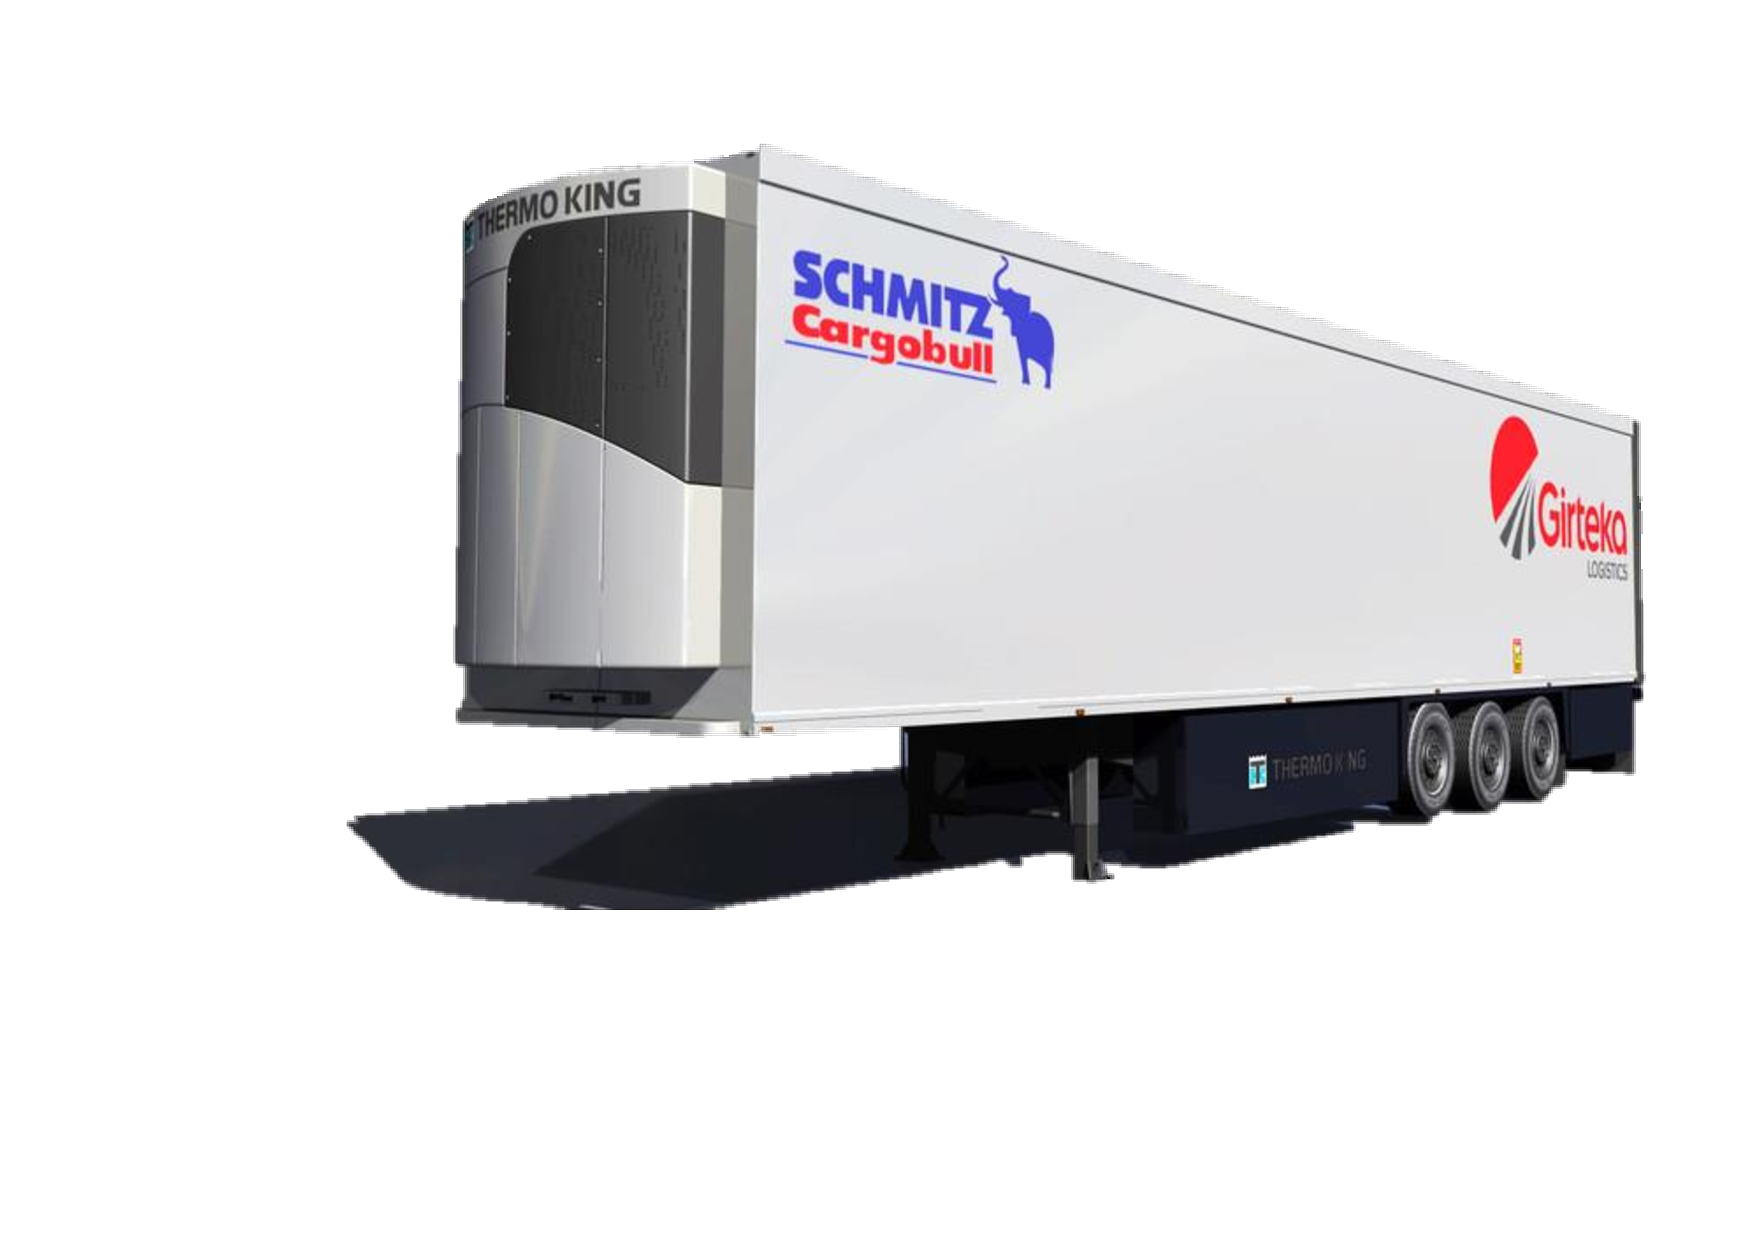
\includegraphics[width=.95\textwidth]{../Graphics/3d_draw_trailer.pdf}
				\centering
				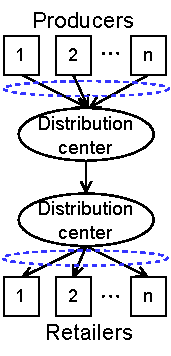
\includegraphics[width=0.45\textwidth]{../Graphics/Transportation_networks.pdf}
 		\end{column}
 	\end{columns}	
\end{frame}

%%%%%%%%%%%%%%%%

\begin{frame}{Introduction}{Problem Motivation and Definition}
	\begin{itemize}
		\item Increased energy efficiency $\rightarrow$ less power required $\rightarrow$ reduced operational costs  
		\item Smaller batteries $\rightarrow$ reduced capital costs		
	\end{itemize}
	\textbf{Efficiency of Reefer Trailers: UN's Sustainable Development Goals}
	\begin{itemize}	
		\item 2nd: Food supply
		\begin{itemize}
			\item Cost of fresh food is correlated with transport costs
			\item Reduced costs increase access to fresh foods for low income people		
		\end{itemize}
		\item 7th: Energy efficiency
		\begin{itemize}
			\item Decreased CO2 emissions per transported good
			\item Decreased use of rare metals for batteries	
		\end{itemize}
	\end{itemize}	
\end{frame}

%%%%%%%%%%%%%%%%%
\begin{frame}{Introduction}{Concept of Reefer trailer}
	\textbf{Some text}
	\begin{itemize}
		\item Insulated trailer
		\item Heat need be removed from cargo through airflow	
	\end{itemize}
	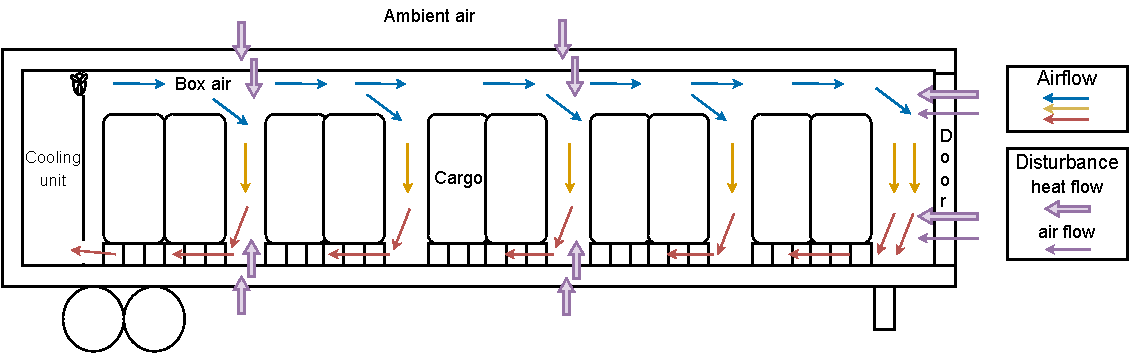
\includegraphics[width=1\textwidth]{../Graphics/Trailer_airflow.pdf}
	\begin{itemize}
		\item High-Fidelity (Hi-Fi) simulation model of trailer is supplied by BITZER
		\item Hi-Fi model is implemented with PID controllers
	\end{itemize}
\end{frame}

%%%%%%%%%%%%%%%%%
\begin{frame}{Introduction}{Problem Definition}
	\textbf{Problem Definition:} Can a MIMO controller be designed to improve energy efficiency of the reefer trailer Hi-Fi simulation model?
\end{frame}

%%%%%%%%%%%%%%%%%
\begin{frame}{System description}{}
	\textbf{Some text}
	\begin{itemize}
		\item Item
	\end{itemize}
\end{frame}

%%%%%%%%%%%%%%%%%
\begin{frame}{System description}{}
	\textbf{Some text}
	\begin{itemize}
		\item Item
	\end{itemize}
\end{frame}

%%%%%%%%%%%%%%%%%
\begin{frame}{System description}{}
	\textbf{Some text}
	\begin{itemize}
		\item Item
	\end{itemize}
\end{frame}

%%%%%%%%%%%%%%%%%
\begin{frame}{System description}{}
	\textbf{Some text}
	\begin{itemize}
		\item Item
	\end{itemize}
\end{frame}

%%%%%%%%%%%%%%%%%%
%\begin{frame}{Next slide title}{Next slide subtitle}
%	\textbf{Some text}
%	\begin{itemize}
%		\item Item
%	\end{itemize}
%\end{frame}
%
%%%%%%%%%%%%%%%%%%
%\begin{frame}{Next slide title}{Next slide subtitle}
%	\textbf{Some text}
%	\begin{itemize}
%		\item Item
%	\end{itemize}
%\end{frame}
%
%%%%%%%%%%%%%%%%%%
%\begin{frame}{Next slide title}{Next slide subtitle}
%	\textbf{Some text}
%	\begin{itemize}
%		\item Item
%	\end{itemize}
%\end{frame}
%
%%%%%%%%%%%%%%%%%%